\documentclass[tikz, border=10pt]{standalone}
\usetikzlibrary{positioning}
\usepackage{tkz-graph}
\begin{document}
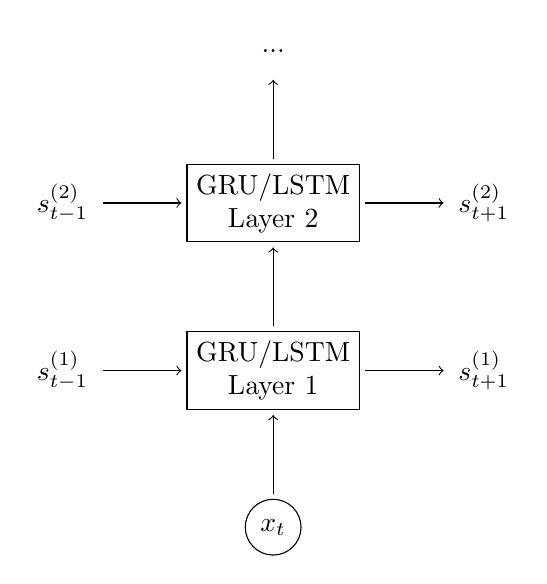
\begin{tikzpicture}

\node[draw, outer sep=2, circle] (x_t) {$x_t$};
\node[draw, align=center, outer sep=2] (unit_t1) [above=of x_t] {GRU/LSTM \\ Layer 1};
\node[draw, align=center, outer sep=2] (unit_t2) [above=of unit_t1] {GRU/LSTM \\ Layer 2};
\node[align=center, outer sep=2] (unit_tprev1) [left=of unit_t1] {$s_{t-1}^{(1)}$};
\node[align=center, outer sep=2] (unit_tnext1) [right=of unit_t1] {$s_{t+1}^{(1)}$};
\node[align=center, outer sep=2] (unit_tprev2) [left=of unit_t2] {$s_{t-1}^{(2)}$};
\node[align=center, outer sep=2] (unit_tnext2) [right=of unit_t2] {$s_{t+1}^{(2)}$};
\node[outer sep=2, circle] (y_t) [above=of unit_t2] {$...$};

\path[->] (x_t) edge (unit_t1);
\path[->] (unit_t1) edge (unit_t2);
\path[->] (unit_t2) edge (y_t);
\path[->] (unit_tprev1) edge (unit_t1);
\path[->] (unit_t1) edge (unit_tnext1);
\path[->] (unit_tprev2) edge (unit_t2);
\path[->] (unit_t2) edge (unit_tnext2);

\end{tikzpicture}
\end{document}
